\documentclass[border=5mm]{standalone}
\usepackage{tikz}

\begin{document}

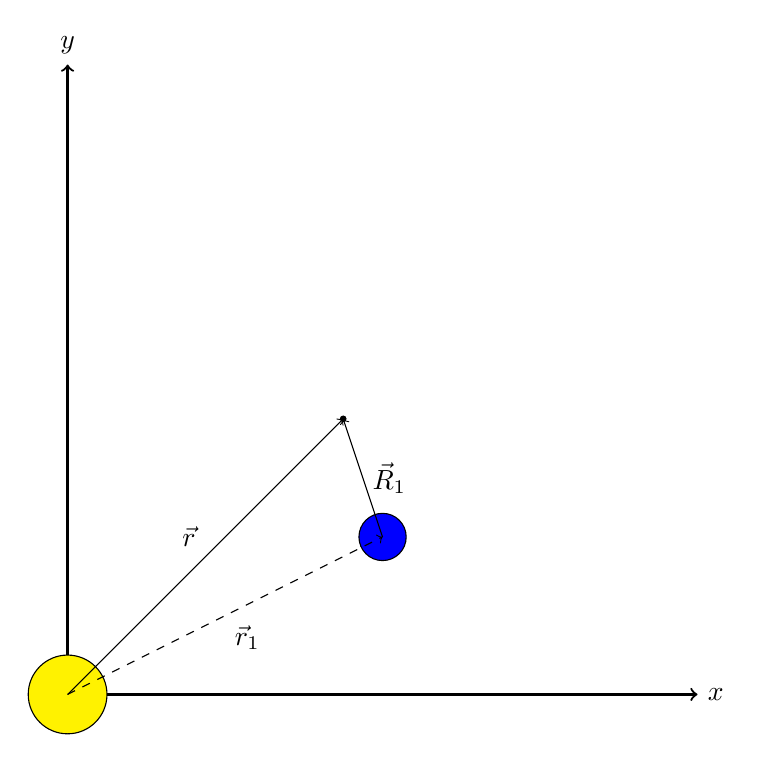
\begin{tikzpicture}

	\draw[thick, ->] (0,0) -- (8,0) node[right]{$x$};
	\draw[thick, ->] (0,0) -- (0,8) node[above]{$y$};
	
	\draw[fill=yellow] (0,0) circle[radius=0.5];
	\draw[fill=blue] (4,2) circle[radius=0.3];
	%\draw[fill=red] (2,6) circle[radius=0.3];
	\draw[fill=black] (3.5,3.5) circle[radius=1pt];
	
	\draw[->] (0,0) -- node[above left]{$\vec{r}$} (3.5,3.5);
	
	\draw[->] (4,2) -- node[right]{$\vec{R}_1$} (3.5,3.5);
	\draw[dashed, ->] (0,0) -- node[below right]{$\vec{r}_1$}(4,2);
	
	%\draw[->] (2,6) -- node[right]{$\vec{R}_2$} (3.5,3.5);
	%\draw[dashed, ->] (0,0) -- node[above left]{$\vec{r}_2$} (2,6);



\end{tikzpicture}



\end{document}